\documentclass[1p]{elsarticle_modified}
%\bibliographystyle{elsarticle-num}

%\usepackage[colorlinks]{hyperref}
%\usepackage{abbrmath_seonhwa} %\Abb, \Ascr, \Acal ,\Abf, \Afrak
\usepackage{amsfonts}
\usepackage{amssymb}
\usepackage{amsmath}
\usepackage{amsthm}
\usepackage{scalefnt}
\usepackage{amsbsy}
\usepackage{kotex}
\usepackage{caption}
\usepackage{subfig}
\usepackage{color}
\usepackage{graphicx}
\usepackage{xcolor} %% white, black, red, green, blue, cyan, magenta, yellow
\usepackage{float}
\usepackage{setspace}
\usepackage{hyperref}

\usepackage{tikz}
\usetikzlibrary{arrows}

\usepackage{multirow}
\usepackage{array} % fixed length table
\usepackage{hhline}

%%%%%%%%%%%%%%%%%%%%%
\makeatletter
\renewcommand*\env@matrix[1][\arraystretch]{%
	\edef\arraystretch{#1}%
	\hskip -\arraycolsep
	\let\@ifnextchar\new@ifnextchar
	\array{*\c@MaxMatrixCols c}}
\makeatother %https://tex.stackexchange.com/questions/14071/how-can-i-increase-the-line-spacing-in-a-matrix
%%%%%%%%%%%%%%%

\usepackage[normalem]{ulem}

\newcommand{\msout}[1]{\ifmmode\text{\sout{\ensuremath{#1}}}\else\sout{#1}\fi}
%SOURCE: \msout is \stkout macro in https://tex.stackexchange.com/questions/20609/strikeout-in-math-mode

\newcommand{\cancel}[1]{
	\ifmmode
	{\color{red}\msout{#1}}
	\else
	{\color{red}\sout{#1}}
	\fi
}

\newcommand{\add}[1]{
	{\color{blue}\uwave{#1}}
}

\newcommand{\replace}[2]{
	\ifmmode
	{\color{red}\msout{#1}}{\color{blue}\uwave{#2}}
	\else
	{\color{red}\sout{#1}}{\color{blue}\uwave{#2}}
	\fi
}

\newcommand{\Sol}{\mathcal{S}} %segment
\newcommand{\D}{D} %diagram
\newcommand{\A}{\mathcal{A}} %arc


%%%%%%%%%%%%%%%%%%%%%%%%%%%%%5 test

\def\sl{\operatorname{\textup{SL}}(2,\Cbb)}
\def\psl{\operatorname{\textup{PSL}}(2,\Cbb)}
\def\quan{\mkern 1mu \triangleright \mkern 1mu}

\theoremstyle{definition}
\newtheorem{thm}{Theorem}[section]
\newtheorem{prop}[thm]{Proposition}
\newtheorem{lem}[thm]{Lemma}
\newtheorem{ques}[thm]{Question}
\newtheorem{cor}[thm]{Corollary}
\newtheorem{defn}[thm]{Definition}
\newtheorem{exam}[thm]{Example}
\newtheorem{rmk}[thm]{Remark}
\newtheorem{alg}[thm]{Algorithm}

\newcommand{\I}{\sqrt{-1}}
\begin{document}

%\begin{frontmatter}
%
%\title{Boundary parabolic representations of knots up to 8 crossings}
%
%%% Group authors per affiliation:
%\author{Yunhi Cho} 
%\address{Department of Mathematics, University of Seoul, Seoul, Korea}
%\ead{yhcho@uos.ac.kr}
%
%
%\author{Seonhwa Kim} %\fnref{s_kim}}
%\address{Center for Geometry and Physics, Institute for Basic Science, Pohang, 37673, Korea}
%\ead{ryeona17@ibs.re.kr}
%
%\author{Hyuk Kim}
%\address{Department of Mathematical Sciences, Seoul National University, Seoul 08826, Korea}
%\ead{hyukkim@snu.ac.kr}
%
%\author{Seokbeom Yoon}
%\address{Department of Mathematical Sciences, Seoul National University, Seoul, 08826,  Korea}
%\ead{sbyoon15@snu.ac.kr}
%
%\begin{abstract}
%We find all boundary parabolic representation of knots up to 8 crossings.
%
%\end{abstract}
%\begin{keyword}
%    \MSC[2010] 57M25 
%\end{keyword}
%
%\end{frontmatter}

%\linenumbers
%\tableofcontents
%
\newcommand\colored[1]{\textcolor{white}{\rule[-0.35ex]{0.8em}{1.4ex}}\kern-0.8em\color{red} #1}%
%\newcommand\colored[1]{\textcolor{white}{ #1}\kern-2.17ex	\textcolor{white}{ #1}\kern-1.81ex	\textcolor{white}{ #1}\kern-2.15ex\color{red}#1	}

{\Large $\underline{12n_{0489}~(K12n_{0489})}$}

\setlength{\tabcolsep}{10pt}
\renewcommand{\arraystretch}{1.6}
\vspace{1cm}\begin{tabular}{m{100pt}>{\centering\arraybackslash}m{274pt}}
\multirow{5}{120pt}{
	\centering
	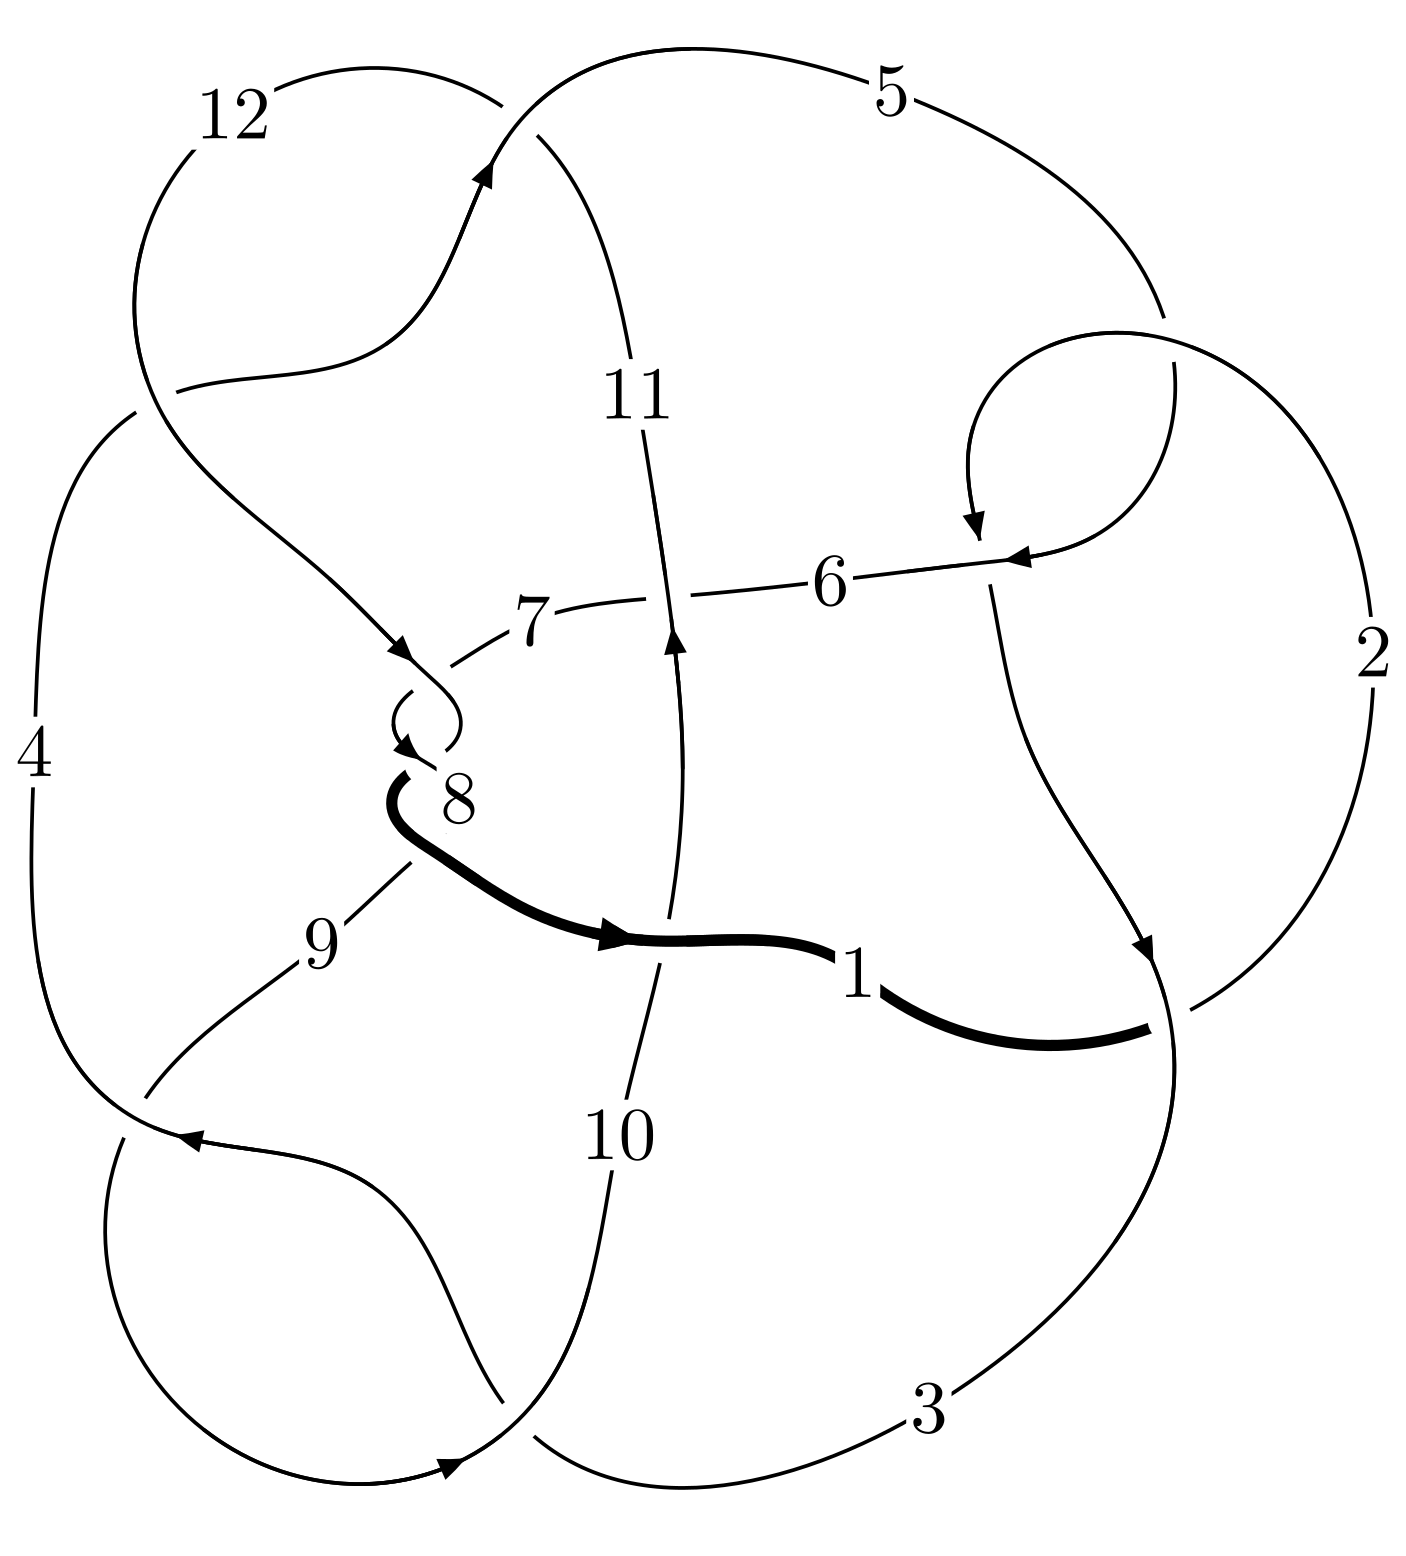
\includegraphics[width=112pt]{../../../GIT/diagram.site/Diagrams/png/2578_12n_0489.png}\\
\ \ \ A knot diagram\footnotemark}&
\allowdisplaybreaks
\textbf{Linearized knot diagam} \\
\cline{2-2}
 &
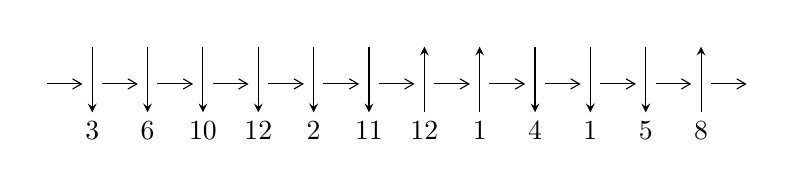
\begin{tikzpicture}[x=20pt, y=17pt]
	% nodes
	\node (C0) at (0, 0) {};
	\node (C1) at (1, 0) {};
	\node (C1U) at (1, +1) {};
	\node (C1D) at (1, -1) {3};

	\node (C2) at (2, 0) {};
	\node (C2U) at (2, +1) {};
	\node (C2D) at (2, -1) {6};

	\node (C3) at (3, 0) {};
	\node (C3U) at (3, +1) {};
	\node (C3D) at (3, -1) {10};

	\node (C4) at (4, 0) {};
	\node (C4U) at (4, +1) {};
	\node (C4D) at (4, -1) {12};

	\node (C5) at (5, 0) {};
	\node (C5U) at (5, +1) {};
	\node (C5D) at (5, -1) {2};

	\node (C6) at (6, 0) {};
	\node (C6U) at (6, +1) {};
	\node (C6D) at (6, -1) {11};

	\node (C7) at (7, 0) {};
	\node (C7U) at (7, +1) {};
	\node (C7D) at (7, -1) {12};

	\node (C8) at (8, 0) {};
	\node (C8U) at (8, +1) {};
	\node (C8D) at (8, -1) {1};

	\node (C9) at (9, 0) {};
	\node (C9U) at (9, +1) {};
	\node (C9D) at (9, -1) {4};

	\node (C10) at (10, 0) {};
	\node (C10U) at (10, +1) {};
	\node (C10D) at (10, -1) {1};

	\node (C11) at (11, 0) {};
	\node (C11U) at (11, +1) {};
	\node (C11D) at (11, -1) {5};

	\node (C12) at (12, 0) {};
	\node (C12U) at (12, +1) {};
	\node (C12D) at (12, -1) {8};
	\node (C13) at (13, 0) {};

	% arrows
	\draw[->,>={angle 60}]
	(C0) edge (C1) (C1) edge (C2) (C2) edge (C3) (C3) edge (C4) (C4) edge (C5) (C5) edge (C6) (C6) edge (C7) (C7) edge (C8) (C8) edge (C9) (C9) edge (C10) (C10) edge (C11) (C11) edge (C12) (C12) edge (C13) ;	\draw[->,>=stealth]
	(C1U) edge (C1D) (C2U) edge (C2D) (C3U) edge (C3D) (C4U) edge (C4D) (C5U) edge (C5D) (C6U) edge (C6D) (C7D) edge (C7U) (C8D) edge (C8U) (C9U) edge (C9D) (C10U) edge (C10D) (C11U) edge (C11D) (C12D) edge (C12U) ;
	\end{tikzpicture} \\
\hhline{~~} \\& 
\textbf{Solving Sequence} \\ \cline{2-2} 
 &
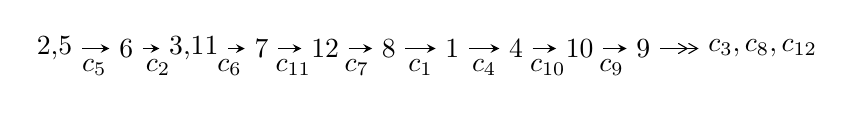
\begin{tikzpicture}[x=23pt, y=7pt]
	% node
	\node (A0) at (-1/8, 0) {2,5};
	\node (A1) at (1, 0) {6};
	\node (A2) at (33/16, 0) {3,11};
	\node (A3) at (25/8, 0) {7};
	\node (A4) at (33/8, 0) {12};
	\node (A5) at (41/8, 0) {8};
	\node (A6) at (49/8, 0) {1};
	\node (A7) at (57/8, 0) {4};
	\node (A8) at (65/8, 0) {10};
	\node (A9) at (73/8, 0) {9};
	\node (C1) at (1/2, -1) {$c_{5}$};
	\node (C2) at (3/2, -1) {$c_{2}$};
	\node (C3) at (21/8, -1) {$c_{6}$};
	\node (C4) at (29/8, -1) {$c_{11}$};
	\node (C5) at (37/8, -1) {$c_{7}$};
	\node (C6) at (45/8, -1) {$c_{1}$};
	\node (C7) at (53/8, -1) {$c_{4}$};
	\node (C8) at (61/8, -1) {$c_{10}$};
	\node (C9) at (69/8, -1) {$c_{9}$};
	\node (A10) at (11, 0) {$c_{3},c_{8},c_{12}$};

	% edge
	\draw[->,>=stealth]	
	(A0) edge (A1) (A1) edge (A2) (A2) edge (A3) (A3) edge (A4) (A4) edge (A5) (A5) edge (A6) (A6) edge (A7) (A7) edge (A8) (A8) edge (A9) ;
	\draw[->>,>={angle 60}]	
	(A9) edge (A10);
\end{tikzpicture} \\ 

\end{tabular} \\

\footnotetext{
The image of knot diagram is generated by the software ``\textbf{Draw programme}" developed by Andrew Bartholomew(\url{http://www.layer8.co.uk/maths/draw/index.htm\#Running-draw}), where we modified some parts for our purpose(\url{https://github.com/CATsTAILs/LinksPainter}).
}\phantom \\ \newline 
\centering \textbf{Ideals for irreducible components\footnotemark of $X_{\text{par}}$} 
 
\begin{align*}
I^u_{1}&=\langle 
-17 u^{26}-87 u^{25}+\cdots+4 b-12,\;47 u^{26}+291 u^{25}+\cdots+8 a+260,\;u^{27}+7 u^{26}+\cdots+44 u+8\rangle \\
I^u_{2}&=\langle 
58848 u^7 a^5+58468 u^7 a^4+\cdots+79844 a+35715,\;2 u^7 a^5+15 u^7 a^4+\cdots+216 a+224,\\
\phantom{I^u_{2}}&\phantom{= \langle  }u^8- u^7- u^6+2 u^5+u^4-2 u^3+2 u-1\rangle \\
I^u_{3}&=\langle 
u^{15}-2 u^{13}+u^{12}+6 u^{11}- u^{10}-8 u^9+4 u^8+11 u^7-3 u^6-8 u^5+4 u^4+6 u^3-2 u^2+b- u,\\
\phantom{I^u_{3}}&\phantom{= \langle  }-2 u^{15}+2 u^{14}+\cdots+a-4,\\
\phantom{I^u_{3}}&\phantom{= \langle  }u^{16}-3 u^{14}+u^{13}+8 u^{12}-2 u^{11}-13 u^{10}+5 u^9+17 u^8-6 u^7-15 u^6+6 u^5+10 u^4-4 u^3-4 u^2+u+1\rangle \\
\\
\end{align*}
\raggedright * 3 irreducible components of $\dim_{\mathbb{C}}=0$, with total 91 representations.\\
\footnotetext{All coefficients of polynomials are rational numbers. But the coefficients are sometimes approximated in decimal forms when there is not enough margin.}
\newpage
\renewcommand{\arraystretch}{1}
\centering \section*{I. $I^u_{1}= \langle -17 u^{26}-87 u^{25}+\cdots+4 b-12,\;47 u^{26}+291 u^{25}+\cdots+8 a+260,\;u^{27}+7 u^{26}+\cdots+44 u+8 \rangle$}
\flushleft \textbf{(i) Arc colorings}\\
\begin{tabular}{m{7pt} m{180pt} m{7pt} m{180pt} }
\flushright $a_{2}=$&$\begin{pmatrix}0\\u\end{pmatrix}$ \\
\flushright $a_{5}=$&$\begin{pmatrix}1\\0\end{pmatrix}$ \\
\flushright $a_{6}=$&$\begin{pmatrix}1\\u^2\end{pmatrix}$ \\
\flushright $a_{3}=$&$\begin{pmatrix}- u\\- u^3+u\end{pmatrix}$ \\
\flushright $a_{11}=$&$\begin{pmatrix}-5.87500 u^{26}-36.3750 u^{25}+\cdots-165.250 u-32.5000\\\frac{17}{4} u^{26}+\frac{87}{4} u^{25}+\cdots+34 u+3\end{pmatrix}$ \\
\flushright $a_{7}=$&$\begin{pmatrix}\frac{53}{8} u^{26}+\frac{301}{8} u^{25}+\cdots+\frac{475}{4} u+21\\-\frac{3}{4} u^{26}-\frac{11}{4} u^{25}+\cdots+\frac{47}{2} u+7\end{pmatrix}$ \\
\flushright $a_{12}=$&$\begin{pmatrix}-10.1250 u^{26}-58.1250 u^{25}+\cdots-199.250 u-35.5000\\\frac{17}{4} u^{26}+\frac{87}{4} u^{25}+\cdots+34 u+3\end{pmatrix}$ \\
\flushright $a_{8}=$&$\begin{pmatrix}-\frac{75}{8} u^{26}-\frac{461}{8} u^{25}+\cdots-\frac{535}{2} u-52\\\frac{15}{2} u^{26}+40 u^{25}+\cdots+\frac{165}{2} u+11\end{pmatrix}$ \\
\flushright $a_{1}=$&$\begin{pmatrix}u^3\\u^5- u^3+u\end{pmatrix}$ \\
\flushright $a_{4}=$&$\begin{pmatrix}\frac{19}{8} u^{26}+\frac{107}{8} u^{25}+\cdots+\frac{245}{4} u+13\\\frac{1}{4} u^{26}+\frac{13}{4} u^{25}+\cdots+\frac{65}{2} u+7\end{pmatrix}$ \\
\flushright $a_{10}=$&$\begin{pmatrix}13.1250 u^{26}+78.6250 u^{25}+\cdots+338.750 u+63.5000\\-\frac{27}{4} u^{26}-\frac{121}{4} u^{25}+\cdots+68 u+25\end{pmatrix}$ \\
\flushright $a_{9}=$&$\begin{pmatrix}\frac{115}{8} u^{26}+\frac{749}{8} u^{25}+\cdots+\frac{1047}{2} u+108\\-17 u^{26}-\frac{185}{2} u^{25}+\cdots-\frac{455}{2} u-35\end{pmatrix}$\\&\end{tabular}
\flushleft \textbf{(ii) Obstruction class $= -1$}\\~\\
\flushleft \textbf{(iii) Cusp Shapes $= -23 u^{26}-150 u^{25}-376 u^{24}-261 u^{23}+729 u^{22}+1734 u^{21}+538 u^{20}-2534 u^{19}-2547 u^{18}+3058 u^{17}+6966 u^{16}+232 u^{15}-11605 u^{14}-12159 u^{13}+2392 u^{12}+15331 u^{11}+11486 u^{10}-2810 u^9-10111 u^8-4910 u^7+3090 u^6+4696 u^5+1095 u^4-1912 u^3-2073 u^2-972 u-214$}\\~\\
\newpage\renewcommand{\arraystretch}{1}
\flushleft \textbf{(iv) u-Polynomials at the component}\newline \\
\begin{tabular}{m{50pt}|m{274pt}}
Crossings & \hspace{64pt}u-Polynomials at each crossing \\
\hline $$\begin{aligned}c_{1}\end{aligned}$$&$\begin{aligned}
&u^{27}+9 u^{26}+\cdots+144 u+64
\end{aligned}$\\
\hline $$\begin{aligned}c_{2},c_{5}\end{aligned}$$&$\begin{aligned}
&u^{27}+7 u^{26}+\cdots+44 u+8
\end{aligned}$\\
\hline $$\begin{aligned}c_{3},c_{4},c_{9}\\c_{11}\end{aligned}$$&$\begin{aligned}
&u^{27}+4 u^{25}+\cdots+3 u+1
\end{aligned}$\\
\hline $$\begin{aligned}c_{6},c_{10}\end{aligned}$$&$\begin{aligned}
&u^{27}-2 u^{26}+\cdots+10 u+1
\end{aligned}$\\
\hline $$\begin{aligned}c_{7},c_{8},c_{12}\end{aligned}$$&$\begin{aligned}
&u^{27}+15 u^{26}+\cdots+2816 u+256
\end{aligned}$\\
\hline
\end{tabular}\\~\\
\newpage\renewcommand{\arraystretch}{1}
\flushleft \textbf{(v) Riley Polynomials at the component}\newline \\
\begin{tabular}{m{50pt}|m{274pt}}
Crossings & \hspace{64pt}Riley Polynomials at each crossing \\
\hline $$\begin{aligned}c_{1}\end{aligned}$$&$\begin{aligned}
&y^{27}+19 y^{26}+\cdots-11008 y-4096
\end{aligned}$\\
\hline $$\begin{aligned}c_{2},c_{5}\end{aligned}$$&$\begin{aligned}
&y^{27}-9 y^{26}+\cdots+144 y-64
\end{aligned}$\\
\hline $$\begin{aligned}c_{3},c_{4},c_{9}\\c_{11}\end{aligned}$$&$\begin{aligned}
&y^{27}+8 y^{26}+\cdots-5 y-1
\end{aligned}$\\
\hline $$\begin{aligned}c_{6},c_{10}\end{aligned}$$&$\begin{aligned}
&y^{27}-18 y^{26}+\cdots+116 y-1
\end{aligned}$\\
\hline $$\begin{aligned}c_{7},c_{8},c_{12}\end{aligned}$$&$\begin{aligned}
&y^{27}-15 y^{26}+\cdots+524288 y-65536
\end{aligned}$\\
\hline
\end{tabular}\\~\\
\newpage\flushleft \textbf{(vi) Complex Volumes and Cusp Shapes}
$$\begin{array}{c|c|c}  
\text{Solutions to }I^u_{1}& \I (\text{vol} + \sqrt{-1}CS) & \text{Cusp shape}\\
 \hline 
\begin{aligned}
u &= -0.685572 + 0.852680 I \\
a &= -0.294505 + 0.463699 I \\
b &= -0.669615 - 0.882383 I\end{aligned}
 & \phantom{-}1.08424 - 3.42475 I & -3.67335 + 3.91434 I \\ \hline\begin{aligned}
u &= -0.685572 - 0.852680 I \\
a &= -0.294505 - 0.463699 I \\
b &= -0.669615 + 0.882383 I\end{aligned}
 & \phantom{-}1.08424 + 3.42475 I & -3.67335 - 3.91434 I \\ \hline\begin{aligned}
u &= -0.627323 + 0.898264 I \\
a &= \phantom{-}0.159682 - 0.346047 I \\
b &= \phantom{-}0.73050 + 1.24655 I\end{aligned}
 & \phantom{-}3.67005 - 10.56210 I & -0.83521 + 5.59011 I \\ \hline\begin{aligned}
u &= -0.627323 - 0.898264 I \\
a &= \phantom{-}0.159682 + 0.346047 I \\
b &= \phantom{-}0.73050 - 1.24655 I\end{aligned}
 & \phantom{-}3.67005 + 10.56210 I & -0.83521 - 5.59011 I \\ \hline\begin{aligned}
u &= -0.237310 + 0.870614 I \\
a &= \phantom{-}0.179034 + 0.342963 I \\
b &= \phantom{-}0.625069 - 0.943841 I\end{aligned}
 & \phantom{-}1.43533 + 6.41550 I & -1.16841 - 7.33424 I \\ \hline\begin{aligned}
u &= -0.237310 - 0.870614 I \\
a &= \phantom{-}0.179034 - 0.342963 I \\
b &= \phantom{-}0.625069 + 0.943841 I\end{aligned}
 & \phantom{-}1.43533 - 6.41550 I & -1.16841 + 7.33424 I \\ \hline\begin{aligned}
u &= \phantom{-}1.098600 + 0.138393 I \\
a &= \phantom{-}1.98959 + 0.36891 I \\
b &= \phantom{-}0.870859 + 0.704449 I\end{aligned}
 & -5.71910 - 3.18007 I & -10.81910 + 3.99905 I \\ \hline\begin{aligned}
u &= \phantom{-}1.098600 - 0.138393 I \\
a &= \phantom{-}1.98959 - 0.36891 I \\
b &= \phantom{-}0.870859 - 0.704449 I\end{aligned}
 & -5.71910 + 3.18007 I & -10.81910 - 3.99905 I \\ \hline\begin{aligned}
u &= \phantom{-}0.693539 + 0.484425 I \\
a &= -0.697012 + 0.794438 I \\
b &= -0.093480 - 0.606899 I\end{aligned}
 & \phantom{-}1.37365 - 1.86319 I & -0.94665 + 4.18320 I \\ \hline\begin{aligned}
u &= \phantom{-}0.693539 - 0.484425 I \\
a &= -0.697012 - 0.794438 I \\
b &= -0.093480 + 0.606899 I\end{aligned}
 & \phantom{-}1.37365 + 1.86319 I & -0.94665 - 4.18320 I\\
 \hline 
 \end{array}$$\newpage$$\begin{array}{c|c|c}  
\text{Solutions to }I^u_{1}& \I (\text{vol} + \sqrt{-1}CS) & \text{Cusp shape}\\
 \hline 
\begin{aligned}
u &= -1.024830 + 0.541180 I \\
a &= \phantom{-}0.720475 + 1.113140 I \\
b &= \phantom{-}0.938303 + 0.355958 I\end{aligned}
 & -3.31479 + 3.49091 I & -9.36494 - 3.65965 I \\ \hline\begin{aligned}
u &= -1.024830 - 0.541180 I \\
a &= \phantom{-}0.720475 - 1.113140 I \\
b &= \phantom{-}0.938303 - 0.355958 I\end{aligned}
 & -3.31479 - 3.49091 I & -9.36494 + 3.65965 I \\ \hline\begin{aligned}
u &= \phantom{-}1.179100 + 0.151427 I \\
a &= -1.68814 - 0.80165 I \\
b &= -0.832047 - 1.051930 I\end{aligned}
 & -3.55373 - 9.54122 I & -7.19005 + 7.47977 I \\ \hline\begin{aligned}
u &= \phantom{-}1.179100 - 0.151427 I \\
a &= -1.68814 + 0.80165 I \\
b &= -0.832047 + 1.051930 I\end{aligned}
 & -3.55373 + 9.54122 I & -7.19005 - 7.47977 I \\ \hline\begin{aligned}
u &= -0.777167\phantom{ +0.000000I} \\
a &= -0.501723\phantom{ +0.000000I} \\
b &= -0.408121\phantom{ +0.000000I}\end{aligned}
 & -1.00831\phantom{ +0.000000I} & -10.7050\phantom{ +0.000000I} \\ \hline\begin{aligned}
u &= -1.143530 + 0.466150 I \\
a &= -0.139215 - 0.916449 I \\
b &= -0.656924 - 0.691492 I\end{aligned}
 & -1.52298 - 1.56653 I & -6.91776 + 4.99160 I \\ \hline\begin{aligned}
u &= -1.143530 - 0.466150 I \\
a &= -0.139215 + 0.916449 I \\
b &= -0.656924 + 0.691492 I\end{aligned}
 & -1.52298 + 1.56653 I & -6.91776 - 4.99160 I \\ \hline\begin{aligned}
u &= -0.916430 + 0.866188 I \\
a &= -0.479520 - 1.066450 I \\
b &= -0.009586 + 0.768274 I\end{aligned}
 & \phantom{-}9.08124 + 3.20872 I & \phantom{-}9.49976 - 1.13015 I \\ \hline\begin{aligned}
u &= -0.916430 - 0.866188 I \\
a &= -0.479520 + 1.066450 I \\
b &= -0.009586 - 0.768274 I\end{aligned}
 & \phantom{-}9.08124 - 3.20872 I & \phantom{-}9.49976 + 1.13015 I \\ \hline\begin{aligned}
u &= -1.036230 + 0.737283 I \\
a &= \phantom{-}1.67104 + 0.91689 I \\
b &= \phantom{-}0.731439 - 0.942909 I\end{aligned}
 & \phantom{-}0.00440 + 9.36453 I & -4.76974 - 8.14508 I\\
 \hline 
 \end{array}$$\newpage$$\begin{array}{c|c|c}  
\text{Solutions to }I^u_{1}& \I (\text{vol} + \sqrt{-1}CS) & \text{Cusp shape}\\
 \hline 
\begin{aligned}
u &= -1.036230 - 0.737283 I \\
a &= \phantom{-}1.67104 - 0.91689 I \\
b &= \phantom{-}0.731439 + 0.942909 I\end{aligned}
 & \phantom{-}0.00440 - 9.36453 I & -4.76974 + 8.14508 I \\ \hline\begin{aligned}
u &= -1.072090 + 0.729726 I \\
a &= -1.92994 - 0.65272 I \\
b &= -0.79138 + 1.29074 I\end{aligned}
 & \phantom{-}2.2965 + 16.5821 I & -2.72249 - 9.74695 I \\ \hline\begin{aligned}
u &= -1.072090 - 0.729726 I \\
a &= -1.92994 + 0.65272 I \\
b &= -0.79138 - 1.29074 I\end{aligned}
 & \phantom{-}2.2965 - 16.5821 I & -2.72249 + 9.74695 I \\ \hline\begin{aligned}
u &= \phantom{-}0.931659 + 0.932655 I \\
a &= \phantom{-}0.416195 - 0.265879 I \\
b &= \phantom{-}0.053666 + 0.840001 I\end{aligned}
 & \phantom{-}9.39926 - 3.40339 I & \phantom{-}4.88512 + 3.93618 I \\ \hline\begin{aligned}
u &= \phantom{-}0.931659 - 0.932655 I \\
a &= \phantom{-}0.416195 + 0.265879 I \\
b &= \phantom{-}0.053666 - 0.840001 I\end{aligned}
 & \phantom{-}9.39926 + 3.40339 I & \phantom{-}4.88512 - 3.93618 I \\ \hline\begin{aligned}
u &= -0.271005 + 0.622370 I \\
a &= -0.406824 - 0.384016 I \\
b &= -0.692744 + 0.470458 I\end{aligned}
 & -1.39292 + 0.87413 I & -6.12461 - 2.84895 I \\ \hline\begin{aligned}
u &= -0.271005 - 0.622370 I \\
a &= -0.406824 + 0.384016 I \\
b &= -0.692744 - 0.470458 I\end{aligned}
 & -1.39292 - 0.87413 I & -6.12461 + 2.84895 I\\
 \hline 
 \end{array}$$\newpage\newpage\renewcommand{\arraystretch}{1}
\centering \section*{II. $I^u_{2}= \langle 58848 u^7 a^5+58468 u^7 a^4+\cdots+79844 a+35715,\;2 u^7 a^5+15 u^7 a^4+\cdots+216 a+224,\;u^8- u^7- u^6+2 u^5+u^4-2 u^3+2 u-1 \rangle$}
\flushleft \textbf{(i) Arc colorings}\\
\begin{tabular}{m{7pt} m{180pt} m{7pt} m{180pt} }
\flushright $a_{2}=$&$\begin{pmatrix}0\\u\end{pmatrix}$ \\
\flushright $a_{5}=$&$\begin{pmatrix}1\\0\end{pmatrix}$ \\
\flushright $a_{6}=$&$\begin{pmatrix}1\\u^2\end{pmatrix}$ \\
\flushright $a_{3}=$&$\begin{pmatrix}- u\\- u^3+u\end{pmatrix}$ \\
\flushright $a_{11}=$&$\begin{pmatrix}a\\-4.54670 a^{5} u^{7}-4.51735 a^{4} u^{7}+\cdots-6.16889 a-2.75941\end{pmatrix}$ \\
\flushright $a_{7}=$&$\begin{pmatrix}2.18697 a^{5} u^{7}+4.03230 a^{4} u^{7}+\cdots+11.1542 a+13.0883\\1.02326 a^{2} u^{7}-0.511628 u^{7}+\cdots+0.139535 a^{2}-1.06977\end{pmatrix}$ \\
\flushright $a_{12}=$&$\begin{pmatrix}4.54670 a^{5} u^{7}+4.51735 a^{4} u^{7}+\cdots+7.16889 a+2.75941\\-4.54670 a^{5} u^{7}-4.51735 a^{4} u^{7}+\cdots-6.16889 a-2.75941\end{pmatrix}$ \\
\flushright $a_{8}=$&$\begin{pmatrix}1.36213 a^{4} u^{7}+1.69103 a^{3} u^{7}+\cdots+4.92691 a+9.32890\\1.10871 a^{4} u^{7}-0.372093 a^{3} u^{7}+\cdots+1.68771 a+2.68964\end{pmatrix}$ \\
\flushright $a_{1}=$&$\begin{pmatrix}u^3\\u^5- u^3+u\end{pmatrix}$ \\
\flushright $a_{4}=$&$\begin{pmatrix}-1.81264 a^{5} u^{7}-4.09101 a^{4} u^{7}+\cdots-8.42162 a-8.29267\\-0.374334 a^{5} u^{7}+0.0587190 a^{4} u^{7}+\cdots-2.73260 a-2.79564\end{pmatrix}$ \\
\flushright $a_{10}=$&$\begin{pmatrix}0.0878467 a^{5} u^{7}-0.620335 a^{4} u^{7}+\cdots-0.431353 a-0.271035\\-3.49648 a^{5} u^{7}-2.67535 a^{4} u^{7}+\cdots-4.68160 a-2.52963\end{pmatrix}$ \\
\flushright $a_{9}=$&$\begin{pmatrix}-2.58379 a^{4} u^{7}-2.84385 a^{3} u^{7}+\cdots-5.32558 a-9.18798\\1.22166 a^{4} u^{7}+2.10631 a^{3} u^{7}+\cdots+0.538206 a-0.140926\end{pmatrix}$\\&\end{tabular}
\flushleft \textbf{(ii) Obstruction class $= -1$}\\~\\
\flushleft \textbf{(iii) Cusp Shapes $= -\frac{113224}{12943} u^7 a^4-\frac{1880}{301} u^7 a^3+\cdots-\frac{2960}{301} a-\frac{312682}{12943}$}\\~\\
\newpage\renewcommand{\arraystretch}{1}
\flushleft \textbf{(iv) u-Polynomials at the component}\newline \\
\begin{tabular}{m{50pt}|m{274pt}}
Crossings & \hspace{64pt}u-Polynomials at each crossing \\
\hline $$\begin{aligned}c_{1}\end{aligned}$$&$\begin{aligned}
&(u^8+3 u^7+7 u^6+10 u^5+11 u^4+10 u^3+6 u^2+4 u+1)^6
\end{aligned}$\\
\hline $$\begin{aligned}c_{2},c_{5}\end{aligned}$$&$\begin{aligned}
&(u^8- u^7- u^6+2 u^5+u^4-2 u^3+2 u-1)^6
\end{aligned}$\\
\hline $$\begin{aligned}c_{3},c_{4},c_{9}\\c_{11}\end{aligned}$$&$\begin{aligned}
&u^{48}+u^{47}+\cdots-164 u+229
\end{aligned}$\\
\hline $$\begin{aligned}c_{6},c_{10}\end{aligned}$$&$\begin{aligned}
&u^{48}-9 u^{47}+\cdots+666 u+661
\end{aligned}$\\
\hline $$\begin{aligned}c_{7},c_{8},c_{12}\end{aligned}$$&$\begin{aligned}
&(u^3- u^2+1)^{16}
\end{aligned}$\\
\hline
\end{tabular}\\~\\
\newpage\renewcommand{\arraystretch}{1}
\flushleft \textbf{(v) Riley Polynomials at the component}\newline \\
\begin{tabular}{m{50pt}|m{274pt}}
Crossings & \hspace{64pt}Riley Polynomials at each crossing \\
\hline $$\begin{aligned}c_{1}\end{aligned}$$&$\begin{aligned}
&(y^8+5 y^7+11 y^6+6 y^5-17 y^4-34 y^3-22 y^2-4 y+1)^6
\end{aligned}$\\
\hline $$\begin{aligned}c_{2},c_{5}\end{aligned}$$&$\begin{aligned}
&(y^8-3 y^7+7 y^6-10 y^5+11 y^4-10 y^3+6 y^2-4 y+1)^6
\end{aligned}$\\
\hline $$\begin{aligned}c_{3},c_{4},c_{9}\\c_{11}\end{aligned}$$&$\begin{aligned}
&y^{48}+27 y^{47}+\cdots+832312 y+52441
\end{aligned}$\\
\hline $$\begin{aligned}c_{6},c_{10}\end{aligned}$$&$\begin{aligned}
&y^{48}+15 y^{47}+\cdots-734396 y+436921
\end{aligned}$\\
\hline $$\begin{aligned}c_{7},c_{8},c_{12}\end{aligned}$$&$\begin{aligned}
&(y^3- y^2+2 y-1)^{16}
\end{aligned}$\\
\hline
\end{tabular}\\~\\
\newpage\flushleft \textbf{(vi) Complex Volumes and Cusp Shapes}
$$\begin{array}{c|c|c}  
\text{Solutions to }I^u_{2}& \I (\text{vol} + \sqrt{-1}CS) & \text{Cusp shape}\\
 \hline 
\begin{aligned}
u &= \phantom{-}0.570868 + 0.730671 I \\
a &= \phantom{-}0.434653 - 0.839070 I \\
b &= \phantom{-}1.149610 + 0.301433 I\end{aligned}
 & \phantom{-}0.87002 + 3.95936 I & -2.92498 - 3.49024 I \\ \hline\begin{aligned}
u &= \phantom{-}0.570868 + 0.730671 I \\
a &= -0.535134 + 0.647465 I \\
b &= -0.636009 - 0.805422 I\end{aligned}
 & \phantom{-}0.87002 - 1.69689 I & -2.92498 + 2.46866 I \\ \hline\begin{aligned}
u &= \phantom{-}0.570868 + 0.730671 I \\
a &= -0.120842 + 0.801190 I \\
b &= \phantom{-}0.538735 - 0.794929 I\end{aligned}
 & \phantom{-}0.87002 - 1.69689 I & -2.92498 + 2.46866 I \\ \hline\begin{aligned}
u &= \phantom{-}0.570868 + 0.730671 I \\
a &= -0.277424 - 0.743391 I \\
b &= -0.544694 + 1.183380 I\end{aligned}
 & \phantom{-}0.87002 + 3.95936 I & -2.92498 - 3.49024 I \\ \hline\begin{aligned}
u &= \phantom{-}0.570868 + 0.730671 I \\
a &= -0.579346 + 0.223976 I \\
b &= -0.004274 + 0.929917 I\end{aligned}
 & \phantom{-}5.00760 + 1.13123 I & \phantom{-}3.60429 - 0.51079 I \\ \hline\begin{aligned}
u &= \phantom{-}0.570868 + 0.730671 I \\
a &= -0.081353 - 0.401232 I \\
b &= \phantom{-}0.676753 - 1.082970 I\end{aligned}
 & \phantom{-}5.00760 + 1.13123 I & \phantom{-}3.60429 - 0.51079 I \\ \hline\begin{aligned}
u &= \phantom{-}0.570868 - 0.730671 I \\
a &= \phantom{-}0.434653 + 0.839070 I \\
b &= \phantom{-}1.149610 - 0.301433 I\end{aligned}
 & \phantom{-}0.87002 - 3.95936 I & -2.92498 + 3.49024 I \\ \hline\begin{aligned}
u &= \phantom{-}0.570868 - 0.730671 I \\
a &= -0.535134 - 0.647465 I \\
b &= -0.636009 + 0.805422 I\end{aligned}
 & \phantom{-}0.87002 + 1.69689 I & -2.92498 - 2.46866 I \\ \hline\begin{aligned}
u &= \phantom{-}0.570868 - 0.730671 I \\
a &= -0.120842 - 0.801190 I \\
b &= \phantom{-}0.538735 + 0.794929 I\end{aligned}
 & \phantom{-}0.87002 + 1.69689 I & -2.92498 - 2.46866 I \\ \hline\begin{aligned}
u &= \phantom{-}0.570868 - 0.730671 I \\
a &= -0.277424 + 0.743391 I \\
b &= -0.544694 - 1.183380 I\end{aligned}
 & \phantom{-}0.87002 - 3.95936 I & -2.92498 + 3.49024 I\\
 \hline 
 \end{array}$$\newpage$$\begin{array}{c|c|c}  
\text{Solutions to }I^u_{2}& \I (\text{vol} + \sqrt{-1}CS) & \text{Cusp shape}\\
 \hline 
\begin{aligned}
u &= \phantom{-}0.570868 - 0.730671 I \\
a &= -0.579346 - 0.223976 I \\
b &= -0.004274 - 0.929917 I\end{aligned}
 & \phantom{-}5.00760 - 1.13123 I & \phantom{-}3.60429 + 0.51079 I \\ \hline\begin{aligned}
u &= \phantom{-}0.570868 - 0.730671 I \\
a &= -0.081353 + 0.401232 I \\
b &= \phantom{-}0.676753 + 1.082970 I\end{aligned}
 & \phantom{-}5.00760 - 1.13123 I & \phantom{-}3.60429 + 0.51079 I \\ \hline\begin{aligned}
u &= -0.855237 + 0.665892 I \\
a &= \phantom{-}0.842747 - 0.830266 I \\
b &= \phantom{-}0.090666 + 0.885994 I\end{aligned}
 & \phantom{-}4.07009 + 5.40662 I & \phantom{-}0.21317 - 6.54740 I \\ \hline\begin{aligned}
u &= -0.855237 + 0.665892 I \\
a &= -0.494638 - 0.291001 I \\
b &= -0.786177 - 1.031780 I\end{aligned}
 & \phantom{-}4.07009 - 0.24963 I & \phantom{-}0.213168 - 0.588510 I \\ \hline\begin{aligned}
u &= -0.855237 + 0.665892 I \\
a &= \phantom{-}1.57064 + 0.15400 I \\
b &= \phantom{-}0.08193 - 1.92144 I\end{aligned}
 & \phantom{-}8.20767 + 2.57849 I & \phantom{-}6.74243 - 3.56796 I \\ \hline\begin{aligned}
u &= -0.855237 + 0.665892 I \\
a &= -1.43317 - 1.40899 I \\
b &= -0.02034 + 1.49548 I\end{aligned}
 & \phantom{-}8.20767 + 2.57849 I & \phantom{-}6.74243 - 3.56796 I \\ \hline\begin{aligned}
u &= -0.855237 + 0.665892 I \\
a &= \phantom{-}2.08795 + 0.67193 I \\
b &= \phantom{-}0.909681 - 0.905479 I\end{aligned}
 & \phantom{-}4.07009 + 5.40662 I & \phantom{-}0.21317 - 6.54740 I \\ \hline\begin{aligned}
u &= -0.855237 + 0.665892 I \\
a &= -2.33228 - 0.49803 I \\
b &= -0.167674 + 0.729716 I\end{aligned}
 & \phantom{-}4.07009 - 0.24963 I & \phantom{-}0.213168 - 0.588510 I \\ \hline\begin{aligned}
u &= -0.855237 - 0.665892 I \\
a &= \phantom{-}0.842747 + 0.830266 I \\
b &= \phantom{-}0.090666 - 0.885994 I\end{aligned}
 & \phantom{-}4.07009 - 5.40662 I & \phantom{-}0.21317 + 6.54740 I \\ \hline\begin{aligned}
u &= -0.855237 - 0.665892 I \\
a &= -0.494638 + 0.291001 I \\
b &= -0.786177 + 1.031780 I\end{aligned}
 & \phantom{-}4.07009 + 0.24963 I & \phantom{-}0.213168 + 0.588510 I\\
 \hline 
 \end{array}$$\newpage$$\begin{array}{c|c|c}  
\text{Solutions to }I^u_{2}& \I (\text{vol} + \sqrt{-1}CS) & \text{Cusp shape}\\
 \hline 
\begin{aligned}
u &= -0.855237 - 0.665892 I \\
a &= \phantom{-}1.57064 - 0.15400 I \\
b &= \phantom{-}0.08193 + 1.92144 I\end{aligned}
 & \phantom{-}8.20767 - 2.57849 I & \phantom{-}6.74243 + 3.56796 I \\ \hline\begin{aligned}
u &= -0.855237 - 0.665892 I \\
a &= -1.43317 + 1.40899 I \\
b &= -0.02034 - 1.49548 I\end{aligned}
 & \phantom{-}8.20767 - 2.57849 I & \phantom{-}6.74243 + 3.56796 I \\ \hline\begin{aligned}
u &= -0.855237 - 0.665892 I \\
a &= \phantom{-}2.08795 - 0.67193 I \\
b &= \phantom{-}0.909681 + 0.905479 I\end{aligned}
 & \phantom{-}4.07009 - 5.40662 I & \phantom{-}0.21317 + 6.54740 I \\ \hline\begin{aligned}
u &= -0.855237 - 0.665892 I \\
a &= -2.33228 + 0.49803 I \\
b &= -0.167674 - 0.729716 I\end{aligned}
 & \phantom{-}4.07009 + 0.24963 I & \phantom{-}0.213168 + 0.588510 I \\ \hline\begin{aligned}
u &= -1.09818\phantom{ +0.000000I} \\
a &= -0.352337 + 1.063250 I \\
b &= -0.390626 + 0.540817 I\end{aligned}
 & -0.454474\phantom{ +0.000000I} & -2.84453 + 0. I\phantom{ +0.000000I} \\ \hline\begin{aligned}
u &= -1.09818\phantom{ +0.000000I} \\
a &= -0.352337 - 1.063250 I \\
b &= -0.390626 - 0.540817 I\end{aligned}
 & -0.454474\phantom{ +0.000000I} & -2.84453 + 0. I\phantom{ +0.000000I} \\ \hline\begin{aligned}
u &= -1.09818\phantom{ +0.000000I} \\
a &= -1.87930 + 0.47836 I \\
b &= -1.035690 + 0.728269 I\end{aligned}
 & -4.59206 - 2.82812 I & -9.37379 + 2.97945 I \\ \hline\begin{aligned}
u &= -1.09818\phantom{ +0.000000I} \\
a &= -1.87930 - 0.47836 I \\
b &= -1.035690 - 0.728269 I\end{aligned}
 & -4.59206 + 2.82812 I & -9.37379 - 2.97945 I \\ \hline\begin{aligned}
u &= -1.09818\phantom{ +0.000000I} \\
a &= \phantom{-}1.61333 + 1.13807 I \\
b &= \phantom{-}0.740815 + 1.063820 I\end{aligned}
 & -4.59206 - 2.82812 I & -9.37379 + 2.97945 I \\ \hline\begin{aligned}
u &= -1.09818\phantom{ +0.000000I} \\
a &= \phantom{-}1.61333 - 1.13807 I \\
b &= \phantom{-}0.740815 - 1.063820 I\end{aligned}
 & -4.59206 + 2.82812 I & -9.37379 - 2.97945 I\\
 \hline 
 \end{array}$$\newpage$$\begin{array}{c|c|c}  
\text{Solutions to }I^u_{2}& \I (\text{vol} + \sqrt{-1}CS) & \text{Cusp shape}\\
 \hline 
\begin{aligned}
u &= \phantom{-}1.031810 + 0.655470 I \\
a &= \phantom{-}0.012794 - 0.843235 I \\
b &= \phantom{-}0.798211 - 0.789739 I\end{aligned}
 & -0.46900 - 3.61542 I & -4.93820 + 2.31472 I \\ \hline\begin{aligned}
u &= \phantom{-}1.031810 + 0.655470 I \\
a &= -0.655325 + 1.142960 I \\
b &= -1.323150 + 0.413843 I\end{aligned}
 & -0.46900 - 9.27166 I & -4.93820 + 8.27362 I \\ \hline\begin{aligned}
u &= \phantom{-}1.031810 + 0.655470 I \\
a &= \phantom{-}1.57349 + 0.39663 I \\
b &= \phantom{-}0.140651 + 0.792574 I\end{aligned}
 & \phantom{-}3.66858 - 6.44354 I & \phantom{-}1.59106 + 5.29417 I \\ \hline\begin{aligned}
u &= \phantom{-}1.031810 + 0.655470 I \\
a &= -1.65798 + 0.26104 I \\
b &= -0.901119 - 0.974313 I\end{aligned}
 & \phantom{-}3.66858 - 6.44354 I & \phantom{-}1.59106 + 5.29417 I \\ \hline\begin{aligned}
u &= \phantom{-}1.031810 + 0.655470 I \\
a &= -1.55331 + 0.89766 I \\
b &= -0.668354 - 1.023270 I\end{aligned}
 & -0.46900 - 3.61542 I & -4.93820 + 2.31472 I \\ \hline\begin{aligned}
u &= \phantom{-}1.031810 + 0.655470 I \\
a &= \phantom{-}2.13206 - 0.70093 I \\
b &= \phantom{-}0.619236 + 1.261980 I\end{aligned}
 & -0.46900 - 9.27166 I & -4.93820 + 8.27362 I \\ \hline\begin{aligned}
u &= \phantom{-}1.031810 - 0.655470 I \\
a &= \phantom{-}0.012794 + 0.843235 I \\
b &= \phantom{-}0.798211 + 0.789739 I\end{aligned}
 & -0.46900 + 3.61542 I & -4.93820 - 2.31472 I \\ \hline\begin{aligned}
u &= \phantom{-}1.031810 - 0.655470 I \\
a &= -0.655325 - 1.142960 I \\
b &= -1.323150 - 0.413843 I\end{aligned}
 & -0.46900 + 9.27166 I & -4.93820 - 8.27362 I \\ \hline\begin{aligned}
u &= \phantom{-}1.031810 - 0.655470 I \\
a &= \phantom{-}1.57349 - 0.39663 I \\
b &= \phantom{-}0.140651 - 0.792574 I\end{aligned}
 & \phantom{-}3.66858 + 6.44354 I & \phantom{-}1.59106 - 5.29417 I \\ \hline\begin{aligned}
u &= \phantom{-}1.031810 - 0.655470 I \\
a &= -1.65798 - 0.26104 I \\
b &= -0.901119 + 0.974313 I\end{aligned}
 & \phantom{-}3.66858 + 6.44354 I & \phantom{-}1.59106 - 5.29417 I\\
 \hline 
 \end{array}$$\newpage$$\begin{array}{c|c|c}  
\text{Solutions to }I^u_{2}& \I (\text{vol} + \sqrt{-1}CS) & \text{Cusp shape}\\
 \hline 
\begin{aligned}
u &= \phantom{-}1.031810 - 0.655470 I \\
a &= -1.55331 - 0.89766 I \\
b &= -0.668354 + 1.023270 I\end{aligned}
 & -0.46900 + 3.61542 I & -4.93820 - 2.31472 I \\ \hline\begin{aligned}
u &= \phantom{-}1.031810 - 0.655470 I \\
a &= \phantom{-}2.13206 + 0.70093 I \\
b &= \phantom{-}0.619236 - 1.261980 I\end{aligned}
 & -0.46900 + 9.27166 I & -4.93820 - 8.27362 I \\ \hline\begin{aligned}
u &= \phantom{-}0.603304\phantom{ +0.000000I} \\
a &= -1.01626 + 1.44968 I \\
b &= -0.374836 - 0.929425 I\end{aligned}
 & \phantom{-}1.06564 - 2.82812 I & -7.40422 + 2.97945 I \\ \hline\begin{aligned}
u &= \phantom{-}0.603304\phantom{ +0.000000I} \\
a &= -1.01626 - 1.44968 I \\
b &= -0.374836 + 0.929425 I\end{aligned}
 & \phantom{-}1.06564 + 2.82812 I & -7.40422 - 2.97945 I \\ \hline\begin{aligned}
u &= \phantom{-}0.603304\phantom{ +0.000000I} \\
a &= -1.03439 + 2.13156 I \\
b &= \phantom{-}0.13210 + 1.44648 I\end{aligned}
 & \phantom{-}5.20322\phantom{ +0.000000I} &                  -6
-0.874953 + 0. 10   I\phantom{ +0.000000I} \\ \hline\begin{aligned}
u &= \phantom{-}0.603304\phantom{ +0.000000I} \\
a &= -1.03439 - 2.13156 I \\
b &= \phantom{-}0.13210 - 1.44648 I\end{aligned}
 & \phantom{-}5.20322\phantom{ +0.000000I} &                  -6
-0.874953 + 0. 10   I\phantom{ +0.000000I} \\ \hline\begin{aligned}
u &= \phantom{-}0.603304\phantom{ +0.000000I} \\
a &= \phantom{-}0.23542 + 3.29584 I \\
b &= \phantom{-}0.474556 + 0.323382 I\end{aligned}
 & \phantom{-}1.06564 - 2.82812 I & -7.40422 + 2.97945 I \\ \hline\begin{aligned}
u &= \phantom{-}0.603304\phantom{ +0.000000I} \\
a &= \phantom{-}0.23542 - 3.29584 I \\
b &= \phantom{-}0.474556 - 0.323382 I\end{aligned}
 & \phantom{-}1.06564 + 2.82812 I & -7.40422 - 2.97945 I\\
 \hline 
 \end{array}$$\newpage\newpage\renewcommand{\arraystretch}{1}
\centering \section*{III. $I^u_{3}= \langle u^{15}-2 u^{13}+\cdots+b- u,\;-2 u^{15}+2 u^{14}+\cdots+a-4,\;u^{16}-3 u^{14}+\cdots+u+1 \rangle$}
\flushleft \textbf{(i) Arc colorings}\\
\begin{tabular}{m{7pt} m{180pt} m{7pt} m{180pt} }
\flushright $a_{2}=$&$\begin{pmatrix}0\\u\end{pmatrix}$ \\
\flushright $a_{5}=$&$\begin{pmatrix}1\\0\end{pmatrix}$ \\
\flushright $a_{6}=$&$\begin{pmatrix}1\\u^2\end{pmatrix}$ \\
\flushright $a_{3}=$&$\begin{pmatrix}- u\\- u^3+u\end{pmatrix}$ \\
\flushright $a_{11}=$&$\begin{pmatrix}2 u^{15}-2 u^{14}+\cdots-17 u^2+4\\- u^{15}+2 u^{13}+\cdots+2 u^2+u\end{pmatrix}$ \\
\flushright $a_{7}=$&$\begin{pmatrix}- u^{15}+2 u^{14}+\cdots-5 u+1\\u^{13}-2 u^{11}+u^{10}+5 u^9- u^8-6 u^7+3 u^6+6 u^5-2 u^4-3 u^3+2 u^2+u-1\end{pmatrix}$ \\
\flushright $a_{12}=$&$\begin{pmatrix}3 u^{15}-2 u^{14}+\cdots- u+4\\- u^{15}+2 u^{13}+\cdots+2 u^2+u\end{pmatrix}$ \\
\flushright $a_{8}=$&$\begin{pmatrix}2 u^{15}-6 u^{13}+\cdots-2 u+4\\u^{14}+u^{13}+\cdots- u-2\end{pmatrix}$ \\
\flushright $a_{1}=$&$\begin{pmatrix}u^3\\u^5- u^3+u\end{pmatrix}$ \\
\flushright $a_{4}=$&$\begin{pmatrix}-2 u^{15}+6 u^{13}+\cdots+4 u-2\\- u^{14}+3 u^{12}+\cdots+2 u+2\end{pmatrix}$ \\
\flushright $a_{10}=$&$\begin{pmatrix}2 u^{15}-2 u^{14}+\cdots+u+4\\- u^{15}+2 u^{13}+\cdots+u-1\end{pmatrix}$ \\
\flushright $a_{9}=$&$\begin{pmatrix}2 u^{15}-6 u^{13}+\cdots-2 u+4\\u^{14}+u^{13}+\cdots- u-3\end{pmatrix}$\\&\end{tabular}
\flushleft \textbf{(ii) Obstruction class $= 1$}\\~\\
\flushleft \textbf{(iii) Cusp Shapes $= -4 u^{15}+11 u^{14}+12 u^{13}-34 u^{12}-20 u^{11}+84 u^{10}+32 u^9-132 u^8-18 u^7+158 u^6+10 u^5-120 u^4+9 u^3+70 u^2-11 u-17$}\\~\\
\newpage\renewcommand{\arraystretch}{1}
\flushleft \textbf{(iv) u-Polynomials at the component}\newline \\
\begin{tabular}{m{50pt}|m{274pt}}
Crossings & \hspace{64pt}u-Polynomials at each crossing \\
\hline $$\begin{aligned}c_{1}\end{aligned}$$&$\begin{aligned}
&u^{16}-6 u^{15}+\cdots-9 u+1
\end{aligned}$\\
\hline $$\begin{aligned}c_{2}\end{aligned}$$&$\begin{aligned}
&u^{16}-3 u^{14}+\cdots- u+1
\end{aligned}$\\
\hline $$\begin{aligned}c_{3},c_{11}\end{aligned}$$&$\begin{aligned}
&u^{16}+8 u^{14}+\cdots- u+1
\end{aligned}$\\
\hline $$\begin{aligned}c_{4},c_{9}\end{aligned}$$&$\begin{aligned}
&u^{16}+8 u^{14}+\cdots+u+1
\end{aligned}$\\
\hline $$\begin{aligned}c_{5}\end{aligned}$$&$\begin{aligned}
&u^{16}-3 u^{14}+\cdots+u+1
\end{aligned}$\\
\hline $$\begin{aligned}c_{6},c_{10}\end{aligned}$$&$\begin{aligned}
&u^{16}+4 u^{15}+\cdots+8 u+3
\end{aligned}$\\
\hline $$\begin{aligned}c_{7},c_{8}\end{aligned}$$&$\begin{aligned}
&u^{16}+4 u^{15}+\cdots-6 u^2+1
\end{aligned}$\\
\hline $$\begin{aligned}c_{12}\end{aligned}$$&$\begin{aligned}
&u^{16}-4 u^{15}+\cdots-6 u^2+1
\end{aligned}$\\
\hline
\end{tabular}\\~\\
\newpage\renewcommand{\arraystretch}{1}
\flushleft \textbf{(v) Riley Polynomials at the component}\newline \\
\begin{tabular}{m{50pt}|m{274pt}}
Crossings & \hspace{64pt}Riley Polynomials at each crossing \\
\hline $$\begin{aligned}c_{1}\end{aligned}$$&$\begin{aligned}
&y^{16}+14 y^{15}+\cdots+7 y+1
\end{aligned}$\\
\hline $$\begin{aligned}c_{2},c_{5}\end{aligned}$$&$\begin{aligned}
&y^{16}-6 y^{15}+\cdots-9 y+1
\end{aligned}$\\
\hline $$\begin{aligned}c_{3},c_{4},c_{9}\\c_{11}\end{aligned}$$&$\begin{aligned}
&y^{16}+16 y^{15}+\cdots+11 y+1
\end{aligned}$\\
\hline $$\begin{aligned}c_{6},c_{10}\end{aligned}$$&$\begin{aligned}
&y^{16}+6 y^{15}+\cdots+14 y+9
\end{aligned}$\\
\hline $$\begin{aligned}c_{7},c_{8},c_{12}\end{aligned}$$&$\begin{aligned}
&y^{16}-14 y^{15}+\cdots-12 y+1
\end{aligned}$\\
\hline
\end{tabular}\\~\\
\newpage\flushleft \textbf{(vi) Complex Volumes and Cusp Shapes}
$$\begin{array}{c|c|c}  
\text{Solutions to }I^u_{3}& \I (\text{vol} + \sqrt{-1}CS) & \text{Cusp shape}\\
 \hline 
\begin{aligned}
u &= \phantom{-}0.697088 + 0.669632 I \\
a &= \phantom{-}0.872141 - 0.419345 I \\
b &= \phantom{-}0.555602 - 0.792024 I\end{aligned}
 & \phantom{-}3.31760 + 1.95723 I & -1.91125 - 3.50456 I \\ \hline\begin{aligned}
u &= \phantom{-}0.697088 - 0.669632 I \\
a &= \phantom{-}0.872141 + 0.419345 I \\
b &= \phantom{-}0.555602 + 0.792024 I\end{aligned}
 & \phantom{-}3.31760 - 1.95723 I & -1.91125 + 3.50456 I \\ \hline\begin{aligned}
u &= -0.858913 + 0.641497 I \\
a &= \phantom{-}1.57955 + 0.75916 I \\
b &= \phantom{-}0.04461 - 1.68746 I\end{aligned}
 & \phantom{-}7.46435 + 2.50164 I & -6.64418 - 2.34827 I \\ \hline\begin{aligned}
u &= -0.858913 - 0.641497 I \\
a &= \phantom{-}1.57955 - 0.75916 I \\
b &= \phantom{-}0.04461 + 1.68746 I\end{aligned}
 & \phantom{-}7.46435 - 2.50164 I & -6.64418 + 2.34827 I \\ \hline\begin{aligned}
u &= -1.083430 + 0.218721 I \\
a &= \phantom{-}0.063889 - 1.037280 I \\
b &= -0.397891 - 0.465672 I\end{aligned}
 & -0.441697 - 1.082400 I & -2.31411 + 4.80071 I \\ \hline\begin{aligned}
u &= -1.083430 - 0.218721 I \\
a &= \phantom{-}0.063889 + 1.037280 I \\
b &= -0.397891 + 0.465672 I\end{aligned}
 & -0.441697 + 1.082400 I & -2.31411 - 4.80071 I \\ \hline\begin{aligned}
u &= \phantom{-}0.993253 + 0.639630 I \\
a &= -1.76311 + 0.05393 I \\
b &= -0.670393 - 0.715848 I\end{aligned}
 & \phantom{-}2.38716 - 7.06415 I & -5.02024 + 8.84090 I \\ \hline\begin{aligned}
u &= \phantom{-}0.993253 - 0.639630 I \\
a &= -1.76311 - 0.05393 I \\
b &= -0.670393 + 0.715848 I\end{aligned}
 & \phantom{-}2.38716 + 7.06415 I & -5.02024 - 8.84090 I \\ \hline\begin{aligned}
u &= \phantom{-}0.764991 + 0.200725 I \\
a &= -0.19627 - 1.80468 I \\
b &= \phantom{-}0.08665 - 1.47695 I\end{aligned}
 & \phantom{-}5.12690 - 0.82457 I & -2.88269 + 8.96873 I \\ \hline\begin{aligned}
u &= \phantom{-}0.764991 - 0.200725 I \\
a &= -0.19627 + 1.80468 I \\
b &= \phantom{-}0.08665 + 1.47695 I\end{aligned}
 & \phantom{-}5.12690 + 0.82457 I & -2.88269 - 8.96873 I\\
 \hline 
 \end{array}$$\newpage$$\begin{array}{c|c|c}  
\text{Solutions to }I^u_{3}& \I (\text{vol} + \sqrt{-1}CS) & \text{Cusp shape}\\
 \hline 
\begin{aligned}
u &= -0.904876 + 0.830651 I \\
a &= -0.816305 - 0.414345 I \\
b &= \phantom{-}0.015954 + 1.301360 I\end{aligned}
 & \phantom{-}11.24100 + 3.09873 I & \phantom{-}4.47651 - 2.43200 I \\ \hline\begin{aligned}
u &= -0.904876 - 0.830651 I \\
a &= -0.816305 + 0.414345 I \\
b &= \phantom{-}0.015954 - 1.301360 I\end{aligned}
 & \phantom{-}11.24100 - 3.09873 I & \phantom{-}4.47651 + 2.43200 I \\ \hline\begin{aligned}
u &= \phantom{-}0.921176 + 0.893488 I \\
a &= \phantom{-}0.327921 - 0.754564 I \\
b &= \phantom{-}0.029313 + 0.666177 I\end{aligned}
 & \phantom{-}8.63862 - 3.28911 I & -10.02068 + 3.66308 I \\ \hline\begin{aligned}
u &= \phantom{-}0.921176 - 0.893488 I \\
a &= \phantom{-}0.327921 + 0.754564 I \\
b &= \phantom{-}0.029313 - 0.666177 I\end{aligned}
 & \phantom{-}8.63862 + 3.28911 I & -10.02068 - 3.66308 I \\ \hline\begin{aligned}
u &= -0.529286 + 0.266978 I \\
a &= -0.06782 + 2.71225 I \\
b &= \phantom{-}0.336156 - 0.719208 I\end{aligned}
 & \phantom{-}1.74451 + 3.30158 I & \phantom{-}2.81664 - 9.31541 I \\ \hline\begin{aligned}
u &= -0.529286 - 0.266978 I \\
a &= -0.06782 - 2.71225 I \\
b &= \phantom{-}0.336156 + 0.719208 I\end{aligned}
 & \phantom{-}1.74451 - 3.30158 I & \phantom{-}2.81664 + 9.31541 I\\
 \hline 
 \end{array}$$\newpage
\newpage\renewcommand{\arraystretch}{1}
\centering \section*{ IV. u-Polynomials}
\begin{tabular}{m{50pt}|m{274pt}}
Crossings & \hspace{64pt}u-Polynomials at each crossing \\
\hline $$\begin{aligned}c_{1}\end{aligned}$$&$\begin{aligned}
&(u^8+3 u^7+7 u^6+10 u^5+11 u^4+10 u^3+6 u^2+4 u+1)^6\\
&\cdot(u^{16}-6 u^{15}+\cdots-9 u+1)(u^{27}+9 u^{26}+\cdots+144 u+64)
\end{aligned}$\\
\hline $$\begin{aligned}c_{2}\end{aligned}$$&$\begin{aligned}
&((u^8- u^7+\cdots+2 u-1)^{6})(u^{16}-3 u^{14}+\cdots- u+1)\\
&\cdot(u^{27}+7 u^{26}+\cdots+44 u+8)
\end{aligned}$\\
\hline $$\begin{aligned}c_{3},c_{11}\end{aligned}$$&$\begin{aligned}
&(u^{16}+8 u^{14}+\cdots- u+1)(u^{27}+4 u^{25}+\cdots+3 u+1)\\
&\cdot(u^{48}+u^{47}+\cdots-164 u+229)
\end{aligned}$\\
\hline $$\begin{aligned}c_{4},c_{9}\end{aligned}$$&$\begin{aligned}
&(u^{16}+8 u^{14}+\cdots+u+1)(u^{27}+4 u^{25}+\cdots+3 u+1)\\
&\cdot(u^{48}+u^{47}+\cdots-164 u+229)
\end{aligned}$\\
\hline $$\begin{aligned}c_{5}\end{aligned}$$&$\begin{aligned}
&((u^8- u^7+\cdots+2 u-1)^{6})(u^{16}-3 u^{14}+\cdots+u+1)\\
&\cdot(u^{27}+7 u^{26}+\cdots+44 u+8)
\end{aligned}$\\
\hline $$\begin{aligned}c_{6},c_{10}\end{aligned}$$&$\begin{aligned}
&(u^{16}+4 u^{15}+\cdots+8 u+3)(u^{27}-2 u^{26}+\cdots+10 u+1)\\
&\cdot(u^{48}-9 u^{47}+\cdots+666 u+661)
\end{aligned}$\\
\hline $$\begin{aligned}c_{7},c_{8}\end{aligned}$$&$\begin{aligned}
&((u^3- u^2+1)^{16})(u^{16}+4 u^{15}+\cdots-6 u^2+1)\\
&\cdot(u^{27}+15 u^{26}+\cdots+2816 u+256)
\end{aligned}$\\
\hline $$\begin{aligned}c_{12}\end{aligned}$$&$\begin{aligned}
&((u^3- u^2+1)^{16})(u^{16}-4 u^{15}+\cdots-6 u^2+1)\\
&\cdot(u^{27}+15 u^{26}+\cdots+2816 u+256)
\end{aligned}$\\
\hline
\end{tabular}\newpage\renewcommand{\arraystretch}{1}
\centering \section*{ V. Riley Polynomials}
\begin{tabular}{m{50pt}|m{274pt}}
Crossings & \hspace{64pt}Riley Polynomials at each crossing \\
\hline $$\begin{aligned}c_{1}\end{aligned}$$&$\begin{aligned}
&(y^8+5 y^7+11 y^6+6 y^5-17 y^4-34 y^3-22 y^2-4 y+1)^6\\
&\cdot(y^{16}+14 y^{15}+\cdots+7 y+1)(y^{27}+19 y^{26}+\cdots-11008 y-4096)
\end{aligned}$\\
\hline $$\begin{aligned}c_{2},c_{5}\end{aligned}$$&$\begin{aligned}
&(y^8-3 y^7+7 y^6-10 y^5+11 y^4-10 y^3+6 y^2-4 y+1)^6\\
&\cdot(y^{16}-6 y^{15}+\cdots-9 y+1)(y^{27}-9 y^{26}+\cdots+144 y-64)
\end{aligned}$\\
\hline $$\begin{aligned}c_{3},c_{4},c_{9}\\c_{11}\end{aligned}$$&$\begin{aligned}
&(y^{16}+16 y^{15}+\cdots+11 y+1)(y^{27}+8 y^{26}+\cdots-5 y-1)\\
&\cdot(y^{48}+27 y^{47}+\cdots+832312 y+52441)
\end{aligned}$\\
\hline $$\begin{aligned}c_{6},c_{10}\end{aligned}$$&$\begin{aligned}
&(y^{16}+6 y^{15}+\cdots+14 y+9)(y^{27}-18 y^{26}+\cdots+116 y-1)\\
&\cdot(y^{48}+15 y^{47}+\cdots-734396 y+436921)
\end{aligned}$\\
\hline $$\begin{aligned}c_{7},c_{8},c_{12}\end{aligned}$$&$\begin{aligned}
&((y^3- y^2+2 y-1)^{16})(y^{16}-14 y^{15}+\cdots-12 y+1)\\
&\cdot(y^{27}-15 y^{26}+\cdots+524288 y-65536)
\end{aligned}$\\
\hline
\end{tabular}
\vskip 2pc
\end{document}